\documentclass[12pt]{article}
\usepackage[utf8]{inputenc}
\usepackage{amsmath}
\usepackage{graphicx}
\usepackage{float}
\usepackage[margin=1in]{geometry}
\usepackage{lineno}
\setlength{\parskip}{1em}
\renewcommand{\baselinestretch}{1.5}
\newcommand\dbyd[2]{\frac{\mathrm d{#1}}{\mathrm d{#2}}}
\newcommand\dsided[2]{{\mathrm d{#1}}/{\mathrm d{#2}}}
\newcommand{\R}{\mathcal{R}}
\title{Some plots I made to fix/answer some of the problems in my draft}
\author{Roger Zhang}
\date{July 2nd 2018}
\usepackage{color}
\newcommand{\david}[1]{\textcolor{blue}{$\langle${\slshape{\bfseries David:} #1 }$\rangle$}}
\newcommand{\roger}[1]{\textcolor{red}{$\langle${\slshape{\bfseries Roger:} #1 }$\rangle$}}
\usepackage[colorlinks=true,linkcolor=blue]{hyperref}
\newcommand{\pmV}{p_{V}}
\newcommand{\pmI}{p_{I}}
\begin{document}
\maketitle
\clearpage
\section{Dependence of discriminant on proportion of intentional infection ($p$) and basic reproduction number ($\R_0$)}

Here I show several plot with different $\epsilon$ in increasing order.
\subsection{$\epsilon=\frac{7}{29207}$}
\begin{figure}[H]
  \centering
  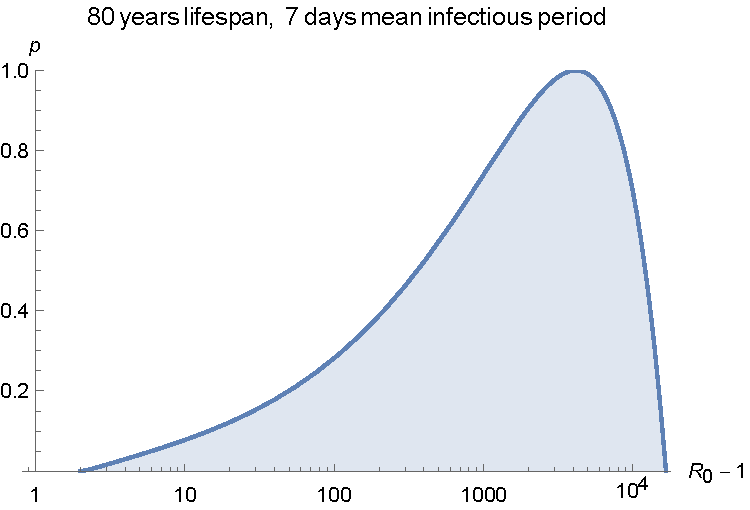
\includegraphics[width=0.9\textwidth]{Figures/80_7.pdf}
\end{figure}

\subsection{$\epsilon=\frac{11}{14611}$}
\begin{figure}[H]
  \centering
  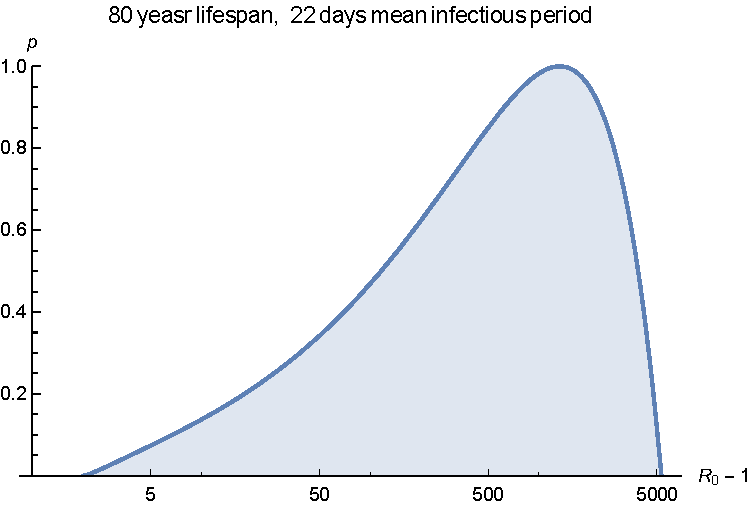
\includegraphics[width=0.9\textwidth]{Figures/80_22.pdf}
\end{figure}

\subsection{$\epsilon=\frac{11}{9136}$}
\begin{figure}[H]
  \centering
  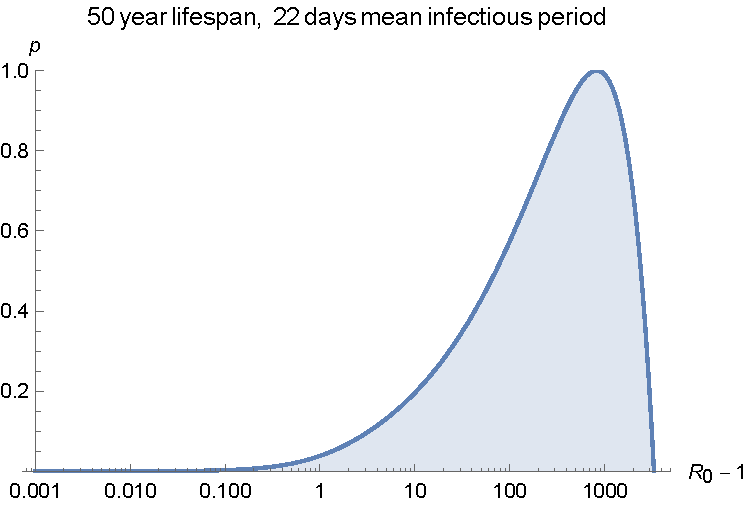
\includegraphics[width=0.9\textwidth]{Figures/50_22.pdf}
\end{figure}

  \subsection{$\epsilon=\frac{1}{81}$}
\begin{figure}[H]
  \centering
  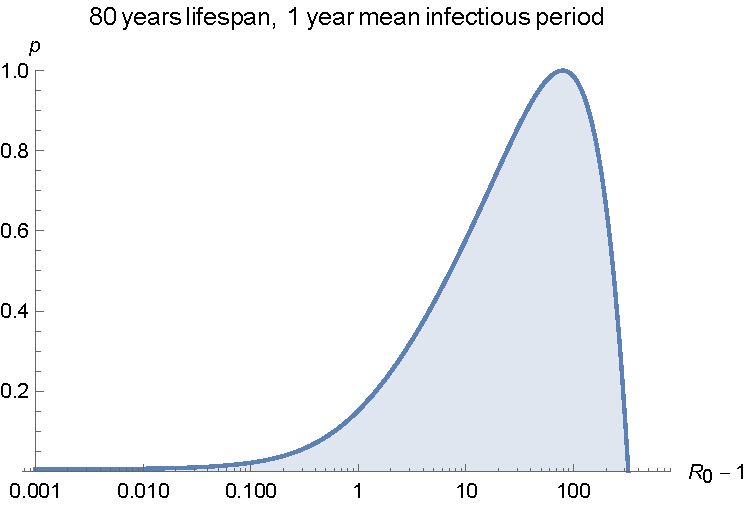
\includegraphics[width=0.9\textwidth]{Figures/80_365.pdf}
\end{figure}
\clearpage

\section{Plot $\epsilon$ as a function of $\R_0$}

Again, I made plots with different $p$ in increasing order
\subsection{$p=0.2$}
\begin{figure}[H]
  \centering
  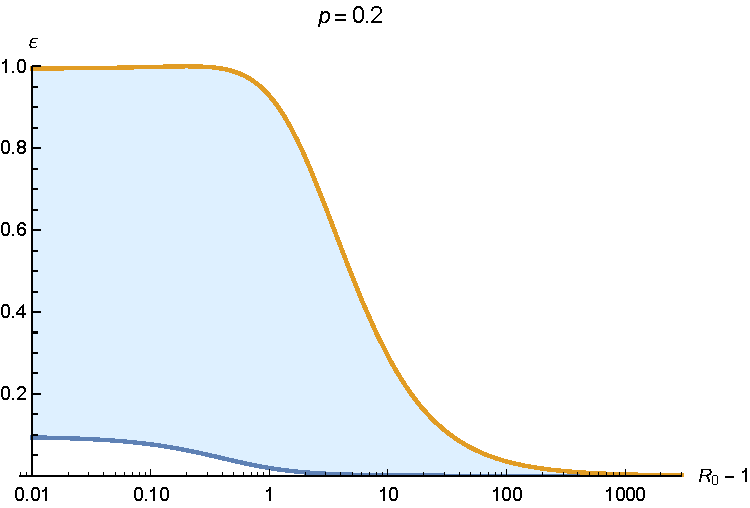
\includegraphics[width=1\textwidth]{Figures/p_0_2.pdf}
\end{figure}

\subsection{$p=0.5$}
\begin{figure}[H]
  \centering
  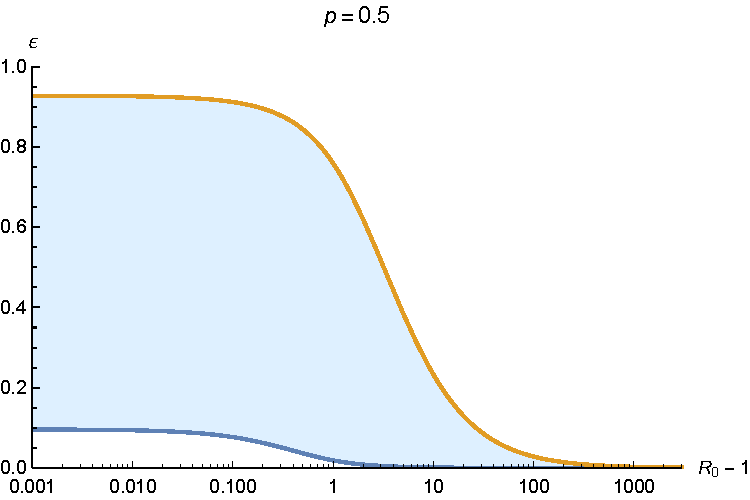
\includegraphics[width=1\textwidth]{Figures/p_0_5.pdf}
\end{figure}

\subsection{$p=0.8$}
\begin{figure}[H]
  \centering
  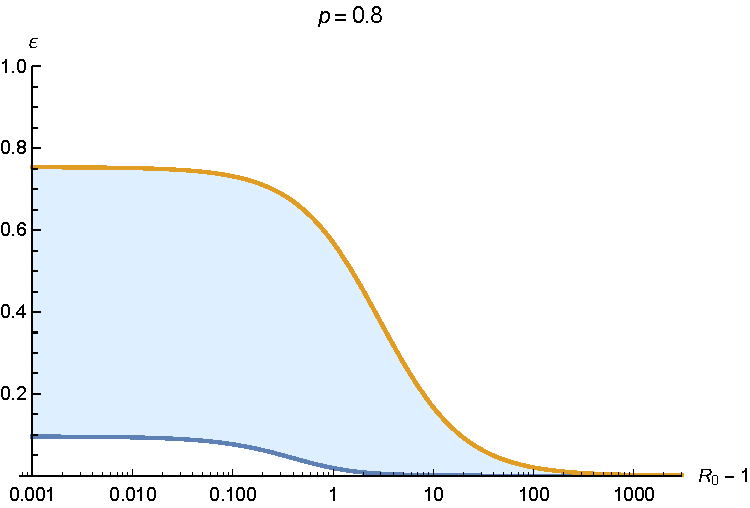
\includegraphics[width=1\textwidth]{Figures/p_0_8.pdf}
\end{figure}
\clearpage
\section{Correct formulation for smallpox and variolation}

We haven't found any evidence suggesting that, individuals infected variolated cases will have different severity of disease from normally infected cases. Here we assume variolation is not by using different strain, but just a different method of infection.

The correct formulation based on this assumption is shown in the following.

\begin{subequations}\label{eq:base_ODE}
\begin{align}
\dbyd{S}{\tau}&=\epsilon(1-p)- \R_0 S(V+I)-\epsilon S\,, \label{eq:S_by_tau}\\
\dbyd{V}{\tau}&=\epsilon p-V\,, \label{eq:V_by_tau}\\
\dbyd{I}{\tau}&=\R_0 SV+\R_0 SI-I\,, \label{eq:I_by_tau}\\
\dbyd{M}{\tau}&=\pmV(1-\epsilon) V+\pmI(1-\epsilon) I\,,\\
\dbyd{R}{\tau}&=(1-\pmV)(1-\epsilon) V+(1-\pmI)(1-\epsilon) I-\epsilon R\,,
\end{align}
\end{subequations}

\subsection{Equilibrium}

By solving the system, we obtain one equilibrium,
\begin{subequations}
\begin{align}
\hat{S}&=\frac{1+\R_0+\sqrt{1-2\R_0+\R_0^2+4p\R_0}}{2\R_0}\,,\\
\hat{V}&=\epsilon p\,,\\
\hat{I}&=\frac{\epsilon}{2}(1-2p-\frac{1}{\R_0}-\frac{\sqrt{1-2\R_0+4p\R_0+\R_0^2}}{\R_0})
\end{align}
\end{subequations}

\end{document}
